\documentclass[english,fleqn,10pt,twocolumn]{article}
\usepackage[utf8]{inputenc}
\usepackage[T1]{fontenc}
\usepackage{babel}
\usepackage{graphics}
\usepackage{cite}

\setlength{\textheight}{23cm}
\setlength{\topmargin}{-0.5cm}
\setlength{\headheight}{0cm}
\setlength{\topskip}{0cm}
\setlength{\columnsep}{1cm}

\setcounter{secnumdepth}{0}

\bibliographystyle{acm}

\date{}
\title{Hardware accelerated ray tracing through OpenGL}
\author{Hanna Reitz\thanks{Faculty of Computer Science, Dresden University of Technology, email: xanclic@googlemail.com}}

\begin{document}

\maketitle

\begin{abstract}
    This paper deals with using standard OpenGL graphics cards (2.1 and up with FBO extension) for hardware acceleration of ray tracing. For this it is necessary to transform the well-known recursive algorithms into iterative ones with
    comparably low execution time complexity. \par
    The result is an algorithm capable of running on today's standard rasterizing graphics hardware in real-time.
\end{abstract}


\section{Introduction}

Ray tracing has been used for long for high-quality 3D image rendering. Compared to the plain rasterization it is much easier parallelizable, however, it also requires heavy parallelization in order to run fast because it operates
independently on every single pixel. Rasterization however may be executed comparably fast also on a single execution unit. This was maybe one of the reasons why early real-time 3D applications (e.g., games) used rasterization instead
of ray tracing. Soon, acceleration hardware was created, featuring rasterization instead of other 3D image rendering techniques.

However, rasterization lacks several features ray tracing includes very easily, such as shadows or reflections and refractions at an arbitrary surface normal. Several techniques have been created in order to circumvent those limitations,
though many are not very intuitive and the others are not very good. Those techniques were soon implemented using parallelized shader units on graphics hardware, because they often worked -- just like ray tracing -- on a per-pixel basis.

Ray tracing remained the standard rendering method for high-quality image generation (especially when used in conjunction with global illumination, which may however be implemented in rasterization, too). In the meantime, rasterizing
became more and more complex while implementing features which ray tracing got all the time. As said before, those resulted in a heavy use of parallel units on graphics hardware, which were soon used for other tasks (GPGPU).
Computation-intense parts of all different kinds of programs are since executed via OpenCL on GPUs.

There are also several attempts of using GPGPU for hardware-accelerated ray tracing (which are closely related to the approach presented in this paper). Others tried to accelerate the ray tracing algorithms itself by optimizing special
use cases (e.g., only triangles as primitives) and thus using modern general-purpose CPUs for real-time rendering. Finally, there were those approaches creating specifically-designed hardware for acceleration, none of which actually
succeeded.

I don't think that specific ray tracing hardware will replace standard graphics cards in the consumer area anytime soon. Furthermore, it is obvious that CPUs are not very suitable for ray tracing. They are designed for all types of
computations, especially single-threaded ones. Ray tracing, on the other hand, does not need most of the capabilities a CPU offers and is nearly arbitrarily parallelizable, directly suggesting GPGPU usage instead.

In conclusion we have to find a way to execute ray tracing on modern graphics hardware whose purpose is strictly speaking rasterizing, but which offer enough parallel computational power to also benefit ray tracing.


\section{General implementation}

As suggested by this paper's title, it will not deal with an OpenCL implementation, but with an OpenGL one. There are (at least) two methods of involving a GPU in the rendering process:
\begin{enumerate}
    \item GPU-assisted: Pass many simple calculations such as matrix multiplications to the GPU, retrieve the output and use the results in mostly on-CPU ray tracing.
    \item Fully GPU-based: Pass all input data (objects, object transformations, etc.) to GPU programs and retrieve the fully-rendered output image.
\end{enumerate}

The first approach may seem simple at the first glance, however, it is not. One has to gather all required calculations (which have to be of the same kind), put them into a texture, read the results back and distribute them -- such a
gathering and distribution system seems rather complicated and will probably be even slower than doing everything right on the CPU. Thus, the only reasonable approach is the second one.

This approach is synchronous multi-threaded. It is obviously multi-threaded, and it is synchronous, because it does one calculation for every pixel and stops after that calculation has been carried out on all of them. A drawback is
that this is not as fast as maybe possible, but it also offers one great advantage when it comes to shadow calculation.

The desired result is now a fully rendered image which does not need any post-processing and may be displayed directly on screen. Hence, every calculation must be executed per pixel and will be executed on every single one.
Every step will thus be carried out via frame buffer objects on textures.


\section{Calculation framework}

At this point, it is obvious that a framework is required to carry out calculations on textures, allowing an arbitrary texture input and output count. The texture count allowed by hardware as input is thus equivalent to the number of
texture image units (samplers per fragment shader), the number of output textures is limited by the minimum of the number of draw buffers and the number of color buffer attachments per frame buffer object.

Calculations will be carried out by fragment shaders. Textures are used as full-size input, the output is written 1-to-1 to other textures. The vertex transformation is hence really simple: It ignores every Z component and just pipes
the input vertex coordinates through so a quad drawn from $(-1, -1)$ to $(1, 1)$ will span the whole output. It will furthermore assign a {\tt uniform vec2} so that it will reach from $(0, 0)$ to $(1, 1)$ (UV coordinates of the input
textures). Other input objects are matrices, vectors and scalars (booleans, floating point numbers, etc.), output is additionally allowed to a combined stencil/depth buffer.

The calculation basically consists of GLSL code, which is split into common (or shared) code, which must be executed for every output object, and specific code describing what to write into which output buffer. For this reason it is
possible to use more output buffers than physically allowed. If using e.g. 13 output buffers with 8 buffers physically allowed per FBO, this framework should create two FBOs with slightly different shader programs, one writing to the
first 8 buffers, the other one accessing the last 5.

The {\tt uniform} mentioned before is used to index the input textures in the fragment shader.

Since the ray tracing itself uses textures, too, the framework should also allow arbitrarily dimensioned textures which may be exchanged at runtime.

Such a framework with all of the described properties has been implemented under the name MACS\footnote{Massive Arbitrary Computations by Shaders}. It is built around a so-called render pass object, which is given the code and all
input and output objects at initialization. The input object values may however be changed at runtime. This design has been chosen to expose the state-machine-like interface of OpenGL, thus improving efficiency.


\section{Ray tracing}

\subsection{Basic input}

The primary input objects are ray maps, one defining the ray starting points and one defining their directions. On the initial ray tracer call they will be initialized to a trivial map representing the rays appropriate for a viewer with
a certain FOV and display aspect.

When doing recursive ray tracing, those initial maps will be replaced by ones generated from the ray tracer itself.

\subsection{Ray tracing}

The first step of ray tracing is to do ray tracing. This is generally implemented by finding the nearest intersection point for every pixel and object available and then returning the object with the minimal intersection distance,
i.e.: Do for every object: Find nearest intersecting object.

This is not reasonably implementable in the given iteration order on hardware, as this would require a list of objects to be present there (which is not impossible, but hard to implement). However, this can be easily fixed by exchanging
the inner and outer itation, i.e.: Do for every object: Find intersection for every pixel and store if nearer than already stored value. There actually is an OpenGL feature which allows exactly that behavior (store if nearer), called
depth testing. Its only drawback is that it requires us to bring every intersection distance into a fixed range, since depth values must be in $[0, 1]$.

Generally, a program is created for every object class which finds the nearest intersection point for a certain ray. It also returns several surface attributes such as the surface normal for that point. Object instances are created by
transforming such a prototype object (e.g. a sphere around the point of origin with radius $1$) by an arbitrary transformation matrix. To transform a ray into the coordinates for the original prototype object, they are basically
multiplied by the inverse of the transformation matrix.

This program writes its result to different output buffers. The intersection distance is divided by a fixed value which is expected to be the the maximum distance, and then written to the depth buffer. The automatic depth testing will
assure that only the object with the minimal intersection distance will be stored in the output buffers. All relevant data will be written to the other buffers: global coordinates of the intersection point, surface normal, surface
tangent and material properties (color, refractive index, etc.).

Each material property may be textured. This is done by another user-defined function which returns a UV coordinate for a given intersection point of the prototype object. This coordinate is then used to index the texture and set the
material attribute value for the respective pixel.

Also, each material property may be freely assigned by a dynamic function (which is what shaders are used for in rasterization). This is really trivial since this is basically equal to texturing, but where the latter uses
{\tt texture2D(texture, uv\_coordinate)}, the completely user-defined function would be called.

In the end, the output buffers contain all surface intersection properties for every pixel there is.

\subsection{Shadowing}

Before applying the lighting, it is necessary to find all shadowed points. In the standard ray tracing model, this is achieved by testing for every pixel and every light source, whether the line in between intersects another object.
However, if one were to implement this directly here, it would probably result in quadratic complexity regarding the object count ($O(n_l \cdot {n_o}^2)$, where $n_o$ is the number of objects and $n_l$ is the number of light sources),
since one would have to check for every object were it is shadowed for every light source over all other objects. This is bad when compared to standard shadowing techniques as used for rasterization, which create all shadows of a light
source by checking every object exactly once ($O(n_l \cdot n_o)$). Every method based off the mentioned one will thus share this disadvantage.

However, in the approach taken here we use the fact that we have the full image available, i.e., every global intersection point is known at this step (in contrast to the standard single-threaded or asynchronous multi-threaded
approach). The method used in here resembles one commonly known as “shadow mapping” for rasterization. This one renders the scene as seen from the light source and uses the resulting depth buffer for determining whether a given surface
is shadowed. Despite being relatively easy to implement and also reasonably fast, it has a major drawback: Since it renders the scene completely independent from the pixels seen by the viewer, the resulting shadows are not very exact.
This can be compensated by using higher resolution textures, which in turn require more video memory and execution time.

Those drawbacks do not apply here. By using ray tracing, one can easily and exactly control which pixels shall be tested for shadowing. The output texture must only be as big as the final output and the resulting shadow map will be
perfect. Other than that, the approach is exactly the same.

For every light source such a shadow map is to be created. For every pixel in the output, a ray (or more specifically: a line) is tested, reaching from the light source to the global intersection point found there. If that line
intersects with anything but the object at its end, the point is considered shadowed. In the end, there will be a shadow map for every light source, which will be used during shading to test whether a given point is affected by a given
light source.

In conclusion, the complexity of this approach is linear again in regard to the object count ($O(n_l \cdot n_o)$).

\subsection{Lighting}

Lighting designates the process of applying incoming light to a surface point. There is not much to be said about this: A light model takes the position of the light source, the position of the lit point, the surface normal and
tangent, the material property and several light properties such as an attenuation function as input. If the given point is affected by the light source (which can be determined by looking at the generated shadow map), a certain
function returns the light intensity reflected by the point to the viewer for every color channel (often, all color channels are calculated simultanously).

The model used in the example implementation is the Schlick model\cite{SCHL93}, which can however be more or less easily replaced by other models such as the Phong model or different ones.

The results of all lighting operations are joined using additive blending.

\subsection{Recursive ray tracing}

Recursive ray tracing enables refraction and reflection. For both phenomenons two new maps have to be generated (ray starting points and directions) which are fed to a recursive call of the hardware ray tracer. The problem to find those
recursive rays is a general ray tracing problem and will thus not be discussed further in here.

There is however an interesting problem: Finding the terminating condition. Normally, one would simply trace until no recursion is necessary anymore or a certain number of recursive calls have been made. Basically this would mean
one would have to do recursive tracing until no pixel needs any recursion anymore (or there are too less). Generally, occlusion queries are ideal for this use case, they did, however, not work for me. The other approach would then be to
carry out a fixed number of recursion levels.

\subsection{Implementation}

The ray tracing algorithm described here is implemented in the Betelgeuse library.


\section{Results}

Of course, the standard ray tracing approach cannot be directly implemented when transforming it into a synchronous multi-threaded model without inherent recursion. Generally, every operation is now executed on all pixels, which means,
one has to generalize data so it can be represented by floating point vectors between iterative steps and that all pixels are always treated exactly the same way (which means one cannot store any special data, such as the intersected
object type).

It is however in fact not too difficult to do this transformation. Every control structure which is not directly possible in a fragment shader such as iteration over a variable list of objects or recursion must simply be taken out of the
shader to the next higher level, which is the program on the CPU calling the shader programs on the GPU.

It was thus possible to create a general ray tracing algorithm with a complexity of $O((n_p \cdot (n_o + n_l \cdot n_o + n_l))^{n_r}) = O((n_l \cdot n_o)^{n_r})$, where
\begin{itemize}
    \item $n_p$ is the number of pixels
    \item $n_o$ is the number of objects
    \item $n_l$ is the number of lights
    \item $n_r$ is the number of recursions (plus one for the initial call)
\end{itemize}

This is exactly the same complexity as for the general ray tracing algorithm. Hence we were able to create an equivalent representation of that algorithm for usage on standard OpenGL 2.1 compatible graphics hardware, which was exactly
the goal set in the first place.

\subsection{Example implementation}

As mentioned in the respective sections, MACS and Betelgeuse together are a sample implementation of the methods mentioned here. MACS implements an interface for carrying out parallel computions on graphics hardware, while Betelgeuse
uses that interface for implementing the ray tracing algorithm described here.

MACS/Betelgeuse proves that the approach taken here is actually applicable and yields the desired results (strong acceleration through OpenGL 2.1 compatible graphics hardware).

\subsection{Comparison}

\subsubsection{One object, two lights}

\begin{figure}[!ht]
    {\centering \resizebox*{3in}{2.5in}{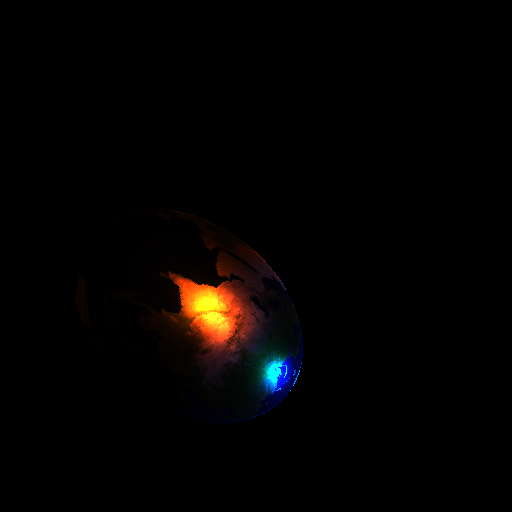
\includegraphics{earth.png}}}
\end{figure}

Rendering time of the given image:
\begin{itemize}
    \item $512 \times 512$:
        \begin{itemize}
            \item 370 ms in a single-threaded software ray tracer, very similar to Betelgeuse (non-textured); single-threaded on a Pentium D with 3.0 GHz
            \item 51.8 FPS (19 ms) on Betelgeuse; on a Radeon X1600
        \end{itemize}
        Speed-up: 19 times
    \item $1024 \times 1024$:
        \begin{itemize}
            \item 1400 ms on CPU
            \item 12.7 FPS (79 ms) on FPU
        \end{itemize}
        Speed-up: 18 times
\end{itemize}

\bibliography{doc}

\end{document}
